\chapter{Results}


\section{Experiments}

\iffalse
SVM-Regression
Random-Forest Regression
Deep Learning Network

Neural Net Sequence Embeddings
One-Hot Encodings
Modfied n-grams skip-grams
\fi

The focus of this research is on the properties of protein owing to its' complex structures. The binding of protein and drug depend on various attributes of protein such as acidity, hydrophobicity, binding pockets and the structure of drug. The attributes are closely related to primary and secondary structure of protein themselves. Therefore, our model aims to relate these multiple components with matrix representation and to confirm to predictions made as per Figure ~\ref{fig:kiba_drug_protein} prediction.

\subsection{Features Selection}
\subsubsection{Primary Feature Selection}
The sequence information of drugs and proteins live in their canonical form. 
% Exploring to the other embedding technique used in language theory, the modified N-Grams Skip-Grams (m-NGSG) was supposed to undertake the mutational agreements when the proteins and drug interaction was brought in question. However, it fared quite badly than the Neural Net Sequence Embeddings. Mostly the issue can be related to that if the algorithm misses the tight relationship among the amino-acid neighborhood, then the protein with different structure may seem to act similarly: a strong disagreement on principle that certain proteins with slight modification on the sequence have different functional and chemical properties. It could still be used for Poisson-Hidden Markov Model for some other properties, but primary encodings can't be relied on m-NGSG. 
Therefore we relied on Neural Net Sequence Embedding technique to form the primary representation. Both protein and drug were converted to Embedding vectors after creation of their labelled encodings. 

\subsubsection{Secondary Features Selection}
These are the structural components of protein especially related to alpha and beta strands of Protein segments. All the protein Sequences are subjected to Equation~(\ref{eq:pssm}) from the labelled encodings. The \acrshort{pssm} matrix is calculated using PSI-BLAST\citep{Schaffer2001}. Then all the testing protein sets are evaluated with the resultant PSSM to form a new PSSM matrix specific to the testing protein. Thus, we expect to explore how proteins relate with the interaction experiments with the protein domain. From the \acrshort{pssm}, we evaluate the other evolutionary and distance vectors using equations \ref{eq:rpt}, \ref{eq:pssmddt}, \ref{eq:pssmsdt} and \ref{eq:edt}.

\subsection{Implementation}
% We explore basically the following algorithms for analyses on protein-drug interactions:


\subsubsection{Stacked Features}
The architecture as per Figure ~\ref{fig:dlm} was implemented for our model design via Python using the TensorFlow framework consisting of keras. The training contained of 200 epochs. The learning rates and early stopping were manipulated in the training process by using keras callback functions. The training and testing was performed using a 5-fold cross-validation set prepared manually. To evaluate the performance of the model, we used concordance index(CI)\citep{Xu2015} as defined by equation~\ref{eq:ci}:
\begin{equation}
    CI = \frac{1}{Z} \sum_{\delta_i > \delta_j} h(b_i - b_j)
    \label{eq:ci}
\end{equation}
where $b_i$ is the prediction value for higher affinity $\delta_i$ and $b_j$ is the prediction value for smallery affinity $\delta_j$, $Z$ is the normalization constant and $h(m)$ is the unit step function:
\begin{equation} h(x) = 
    \begin{cases}
        1,& \quad {if x>0} \\
        0.5, & \quad{ if x=0 } \\
        0, & \quad{if x<0} \\
    \end{cases}
\end{equation}

\section{Results}

The method proposed by this research, \acrfull{featdti} contains 3 \acrfull{cnn}-blocks. It evaluates \acrfull{rpt}, acrfull{edt} and \acrfull{pssmdt} based on the inputs (Protein FASTA and Drugs SMILES) provided. The features are then calculated by the model to calculate the \acrfull{kiba} scores.


% __________________________________________________________________________________________________
% Layer (type)                    Output Shape         Param #     Connected to                     
% ==================================================================================================
% input_10 (InputLayer)           (None, 2000, 1)      0                                            
% __________________________________________________________________________________________________
% input_8 (InputLayer)            (None, 1000)         0                                            
% __________________________________________________________________________________________________
% conv1d_16 (Conv1D)              (None, 1969, 32)     1056        input_10[0][0]                   
% __________________________________________________________________________________________________
% input_7 (InputLayer)            (None, 100)          0                                            
% __________________________________________________________________________________________________
% embedding_4 (Embedding)         (None, 1000, 128)    3328        input_8[0][0]                    
% __________________________________________________________________________________________________
% conv1d_17 (Conv1D)              (None, 1938, 64)     65600       conv1d_16[0][0]                  
% __________________________________________________________________________________________________
% embedding_3 (Embedding)         (None, 100, 128)     8320        input_7[0][0]                    
% __________________________________________________________________________________________________
% conv1d_13 (Conv1D)              (None, 989, 32)      49184       embedding_4[0][0]                
% __________________________________________________________________________________________________
% conv1d_18 (Conv1D)              (None, 1907, 96)     196704      conv1d_17[0][0]                  
% __________________________________________________________________________________________________
% input_11 (InputLayer)           (None, 400, 1)       0                                            
% __________________________________________________________________________________________________
% conv1d_10 (Conv1D)              (None, 97, 32)       16416       embedding_3[0][0]                
% __________________________________________________________________________________________________
% conv1d_14 (Conv1D)              (None, 978, 64)      24640       conv1d_13[0][0]                  
% __________________________________________________________________________________________________
% global_max_pooling1d_10 (Global (None, 96)           0           conv1d_18[0][0]                  
% __________________________________________________________________________________________________
% global_max_pooling1d_11 (Global (None, 1)            0           input_11[0][0]                   
% __________________________________________________________________________________________________
% input_12 (InputLayer)           (None, 400, 1)       0                                            
% __________________________________________________________________________________________________
% conv1d_11 (Conv1D)              (None, 94, 64)       8256        conv1d_10[0][0]                  
% __________________________________________________________________________________________________
% conv1d_15 (Conv1D)              (None, 967, 96)      73824       conv1d_14[0][0]                  
% __________________________________________________________________________________________________
% concatenate_5 (Concatenate)     (None, 97)           0           global_max_pooling1d_10[0][0]    
%                                                                  global_max_pooling1d_11[0][0]    
% __________________________________________________________________________________________________
% global_max_pooling1d_12 (Global (None, 1)            0           input_12[0][0]                   
% __________________________________________________________________________________________________
% conv1d_12 (Conv1D)              (None, 91, 96)       24672       conv1d_11[0][0]                  
% __________________________________________________________________________________________________
% global_max_pooling1d_8 (GlobalM (None, 96)           0           conv1d_15[0][0]                  
% __________________________________________________________________________________________________
% concatenate_6 (Concatenate)     (None, 98)           0           concatenate_5[0][0]              
%                                                                  global_max_pooling1d_12[0][0]    
% __________________________________________________________________________________________________
% global_max_pooling1d_7 (GlobalM (None, 96)           0           conv1d_12[0][0]                  
% __________________________________________________________________________________________________
% concatenate_7 (Concatenate)     (None, 194)          0           global_max_pooling1d_8[0][0]     
%                                                                  concatenate_6[0][0]              
% __________________________________________________________________________________________________
% concatenate_8 (Concatenate)     (None, 290)          0           global_max_pooling1d_7[0][0]     
%                                                                  concatenate_7[0][0]              
% __________________________________________________________________________________________________
% dense_5 (Dense)                 (None, 1024)         297984      concatenate_8[0][0]              
% __________________________________________________________________________________________________
% dropout_3 (Dropout)             (None, 1024)         0           dense_5[0][0]                    
% __________________________________________________________________________________________________
% dense_6 (Dense)                 (None, 1024)         1049600     dropout_3[0][0]                  
% __________________________________________________________________________________________________
% dropout_4 (Dropout)             (None, 1024)         0           dense_6[0][0]                    
% __________________________________________________________________________________________________
% dense_7 (Dense)                 (None, 512)          524800      dropout_4[0][0]                  
% __________________________________________________________________________________________________
% dense_8 (Dense)                 (None, 1)            513         dense_7[0][0]                    
% ==================================================================================================
% Total params: 2,344,897
% Trainable params: 2,344,897
% Non-trainable params: 0

The deep learning method was implemented with various filter sizes of Convolutional Layer of Protein and Drugs. The different sizes were chosen as the lengths of drugs' canonical SMILES sequence and proteins' FASTA sequence differ. Only the comparable results are shown in table \ref{table:results}. The training and validation plots under different settings is clearly shown in Figure \ref{fig:ci_curve}. The different settings described by Figure \ref{fig:train_val} are:
\begin{itemize}
    \item Setting 1 (S1): The validation proteins and drugs appear in training set.
    \item Setting 2 (S2): The validation Protein is seen in training set but validation drugs are not present while training.
    \item Setting 3 (S3): The validation Protein is absent in training set but validation drugs are present in training set.
    \item Setting 4 (S4): The validation Protein and Drugs do not appear in training set.
\end{itemize}

\begin{figure}[tbp]
    \centering
    \subfloat[S1][Setting 1]{
        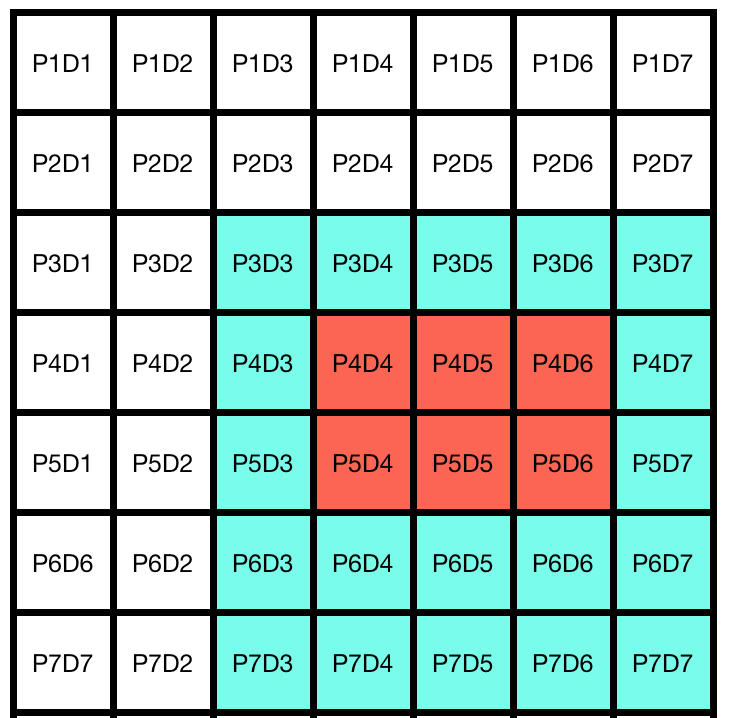
\includegraphics[width=.45\textwidth]{mainmatter/4-Results/images/S1.png}
        \label{fig:s1}
    } \qquad
    \subfloat[S2][Setting 2]{
        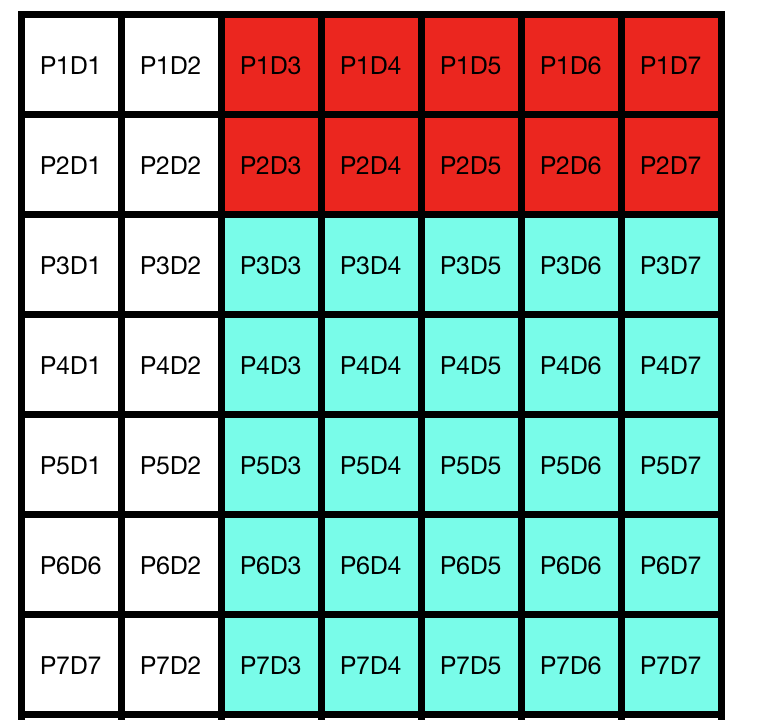
\includegraphics[width=.4\textwidth]{mainmatter/4-Results/images/S2.png}
        \label{fig:s2}
    } \qquad
    \subfloat[S3][Setting 3]{
        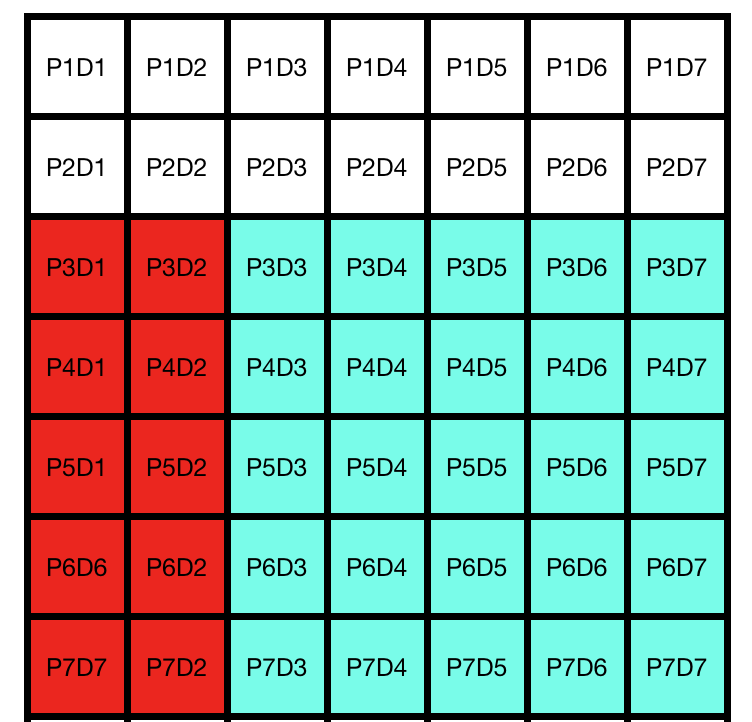
\includegraphics[width=.4\textwidth]{mainmatter/4-Results/images/S3.png}
        \label{fig:s3}
    } \qquad
    \subfloat[S4][Setting 4]{
        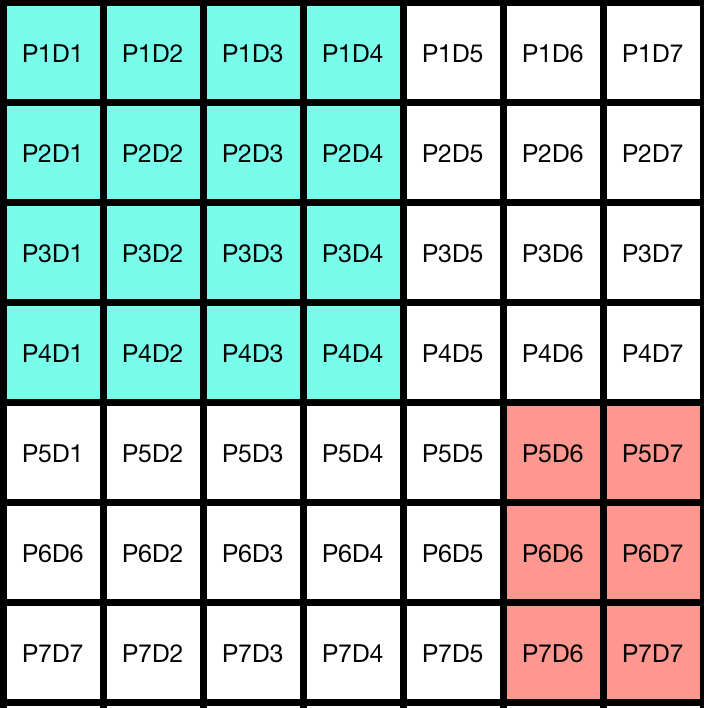
\includegraphics[width=.4\textwidth]{mainmatter/4-Results/images/S4.png}
        \label{fig:s4}
    }
    \caption[Different Settings Of Training and Validation Sets]{Different Settings Of Training and Validation Sets
       \textit{(Brown-Red represents the Validation set and Cyan represents the Training Set)}, Description based on validation Set: \ref{sub@fig:s1} has repeated protein and drugs, \ref{sub@fig:s2} has repeated drugs but unique proteins, \ref{sub@fig:s3} has repeated proteins but unique drugs, and \ref{sub@fig:s4} has unique proteins and drugs.
        }
    \label{fig:train_val}
\end{figure}

\begin{table}[tbp]
    \centering
    \caption[Experiments results under different settings (S1, S2, S3, S4)]{Experiments results under different settings (S1, S2, S3, S4). The model S1 and S4 performed well with same filter size 8 in convolution layer drug-protein. The model S2 performed well with drug filter window of 4 and protein window of 8. The model S3 predicted well with drug window size of 8 and protein window size of 12.}
    \begin{tabular}{|l|c|c|c|c|c|c|}
    \hline 
    
     S.No. & Setting & Drug Smiles & FASTA &  CI-val & MSE  \\ 
       &   & Window Size &  Window Size    & &    \\  \toprule \hline
     1 & S1 & 4 & 8 & 0.813936 & 0.893064 \\ \hline
     2 & S1 & 4 & 12 & 0.810844 & 1.285271 \\ \hline
     3 & S1 & 8 & 8 & 0.873094 & 0.177053 \\ \hline
     4 & S1 & 8 & 12 & 0.807230 & 1.056755 \\ \hline \midrule
      \hline

     1 & S2 & 4 & 8 & 0.788051 & 0.678707 \\ \hline
     2 & S2 & 4 & 12 & 0.802355 & 0.360900 \\ \hline
     3 & S2 & 8 & 8 & 0.803720 & 0.792821 \\ \hline
     4 & S2 & 8 & 12 & 0.803853 & 0.672790 \\ \hline \midrule
      \hline
     1 & S3 & 4 & 8 & 0.815181 & 1.562749 \\ \hline
     2 & S3 & 4 & 12 & 0.805739 & 1.541746 \\ \hline
     3 & S3 & 8 & 8 & 0.813063 & 1.259206 \\ \hline
     4 & S3 & 8 & 12 & 0.824767 & 1.396765 \\ \hline \midrule
      \hline
     1 & S4 & 4 & 8 & 0.803982 & 0.412271 \\ \hline
     2 & S4 & 4 & 12 & 0.805961 & 1.510426 \\ \hline
     3 & S4 & 8 & 8 & 0.815464 & 1.614631 \\ \hline
     4 & S4 & 8 & 12 & 0.787073 & 0.485298 \\ \hline
    \end{tabular}
    \label{table:results}
\end{table}

Here we obtain four different models for prediction of drug and protein interaction. The correct model to choose will depend on type of drug and protein fed into the learning algorithm. To use the correct model, the research work following steps depending on check with input protein FASTA and drug SMILES sequence being fed:
\begin{itemize}
    \item If Both drug and protein are found in the training dataset, use model S1 to predict the KIBA score.
    \item If drug is not found but protein is found in training dataset, use model S2 to predict the KIBA score.
    \item If protein is found but drug is not found in training dataset, use model S3 to predict the KIBA score.
    \item If none of the proteins or drugs is found in training dataset, use model S4 to predict the KIBA score.
\end{itemize}

\subsubsection{Performance of optimizers in Setting 1}

The values obtained by using different optimizers is shown in table \ref{table:optimizer} and Figure \ref{fig:optimizer_plot}. It shows that Adam optimizer exhibits the best optimizer results in comparison to Stochastic Gradient Descent, Adagrad and RMSProp. In fact the other optimizers perform quite poorly compared to Adam optimizer. The learning factor was lowered by using callback ReduceLROnPlateau by a factor of 0.2 when the validation loss didn't increase in 5 consecutive epochs.

\begin{table} [H]
    \centering
    \caption[Scores of different Optimizer] {Scores obtained using other optimizers}
    \label{table:optimizer}
    \begin{tabular}{|l|l|l|}
        \hline
        
        Selection of Optimizer & CI-Index & MSE \\ \toprule 
        
        \hline
        SGD & 0.1087 & 5.320060 \\ \hline
        Adagrad & 0.749753 & 2.202080 \\ \hline
        RMSProp & 0.748766 & 2.202080 \\ \hline
        Adam    & 0.873094 & 0.177053 \\ \hline
        
    \end{tabular}
    
\end{table}

\begin{figure}[htbp]
    \subfloat[][Concordance Index]{
        \label{fig:opt-ci}
        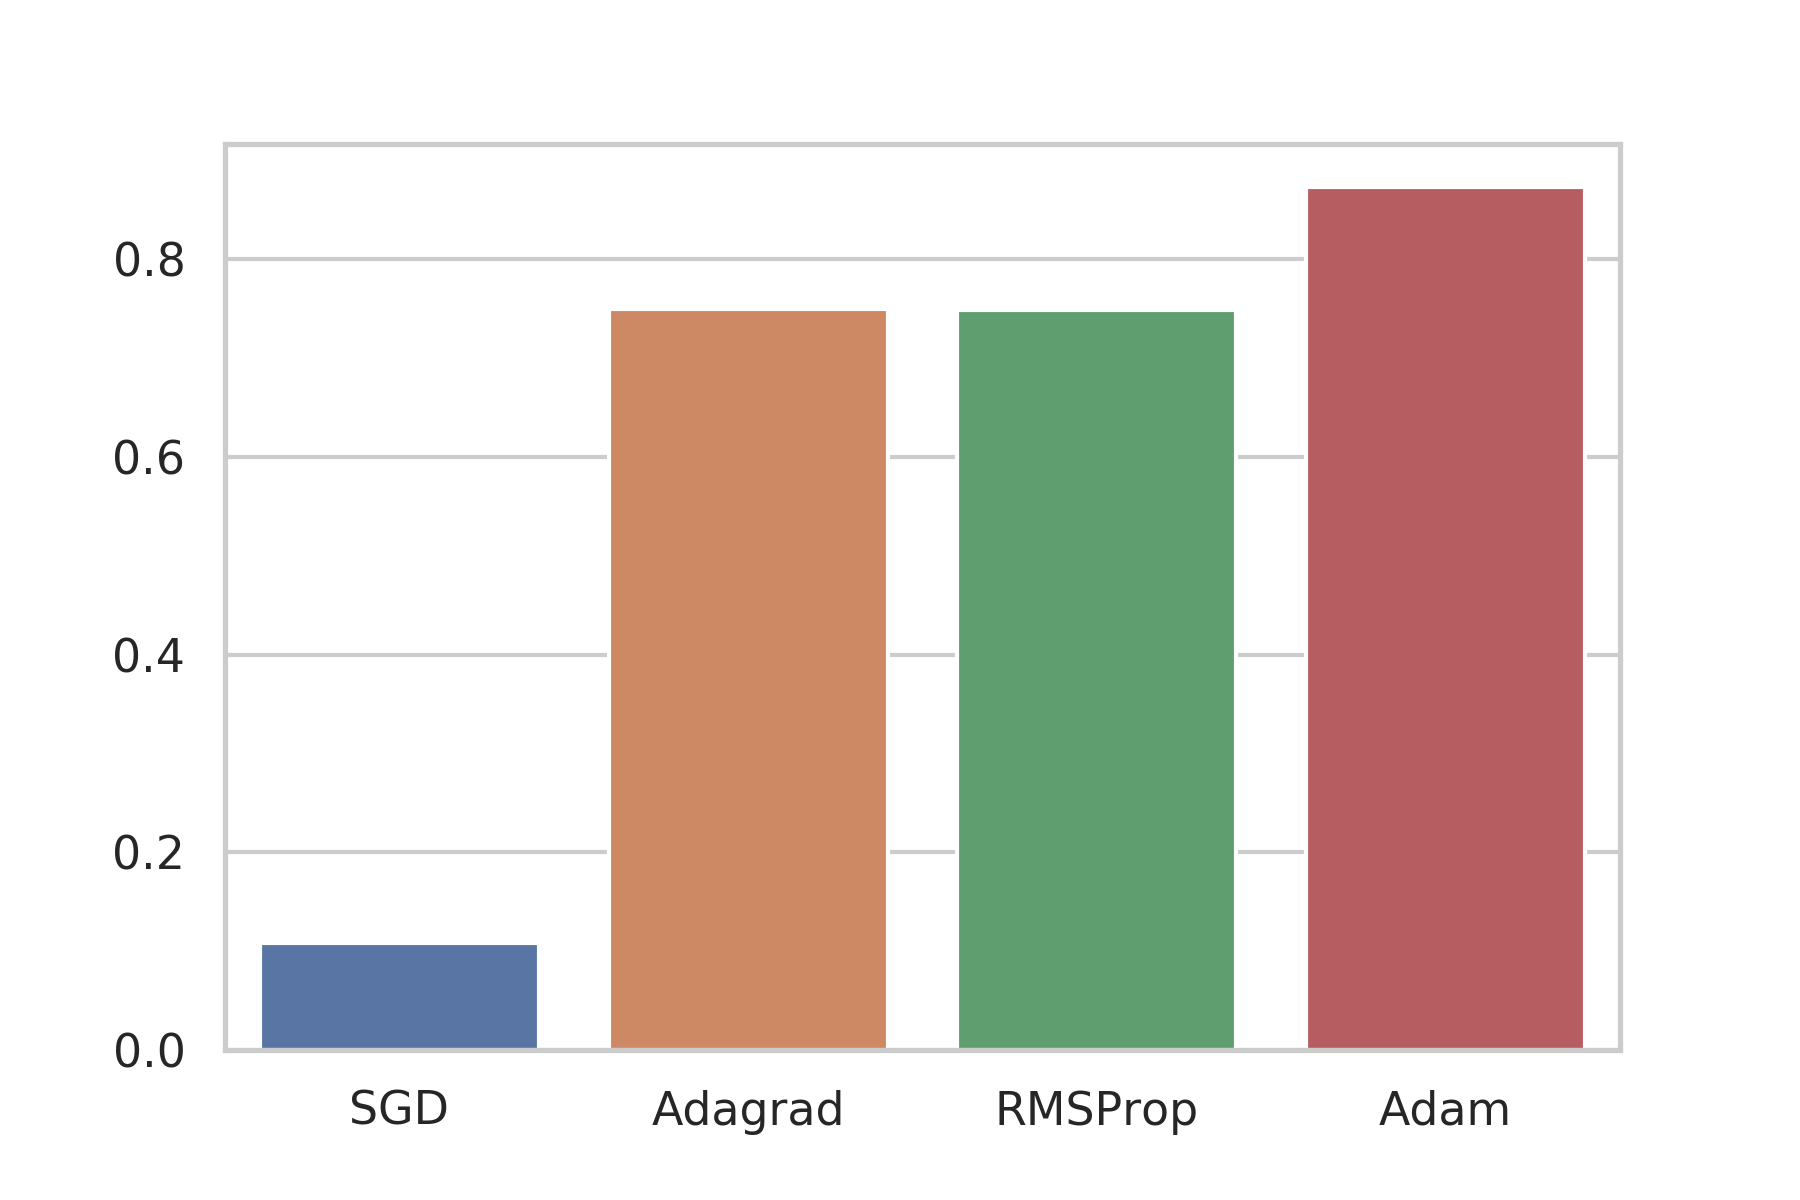
\includegraphics[width=.46\textwidth]{mainmatter/4-Results/images/Experiment_optimizer-CI.png}}\quad
    \subfloat[][Mean Square Error]{
        \label{fig:opt-mse}
        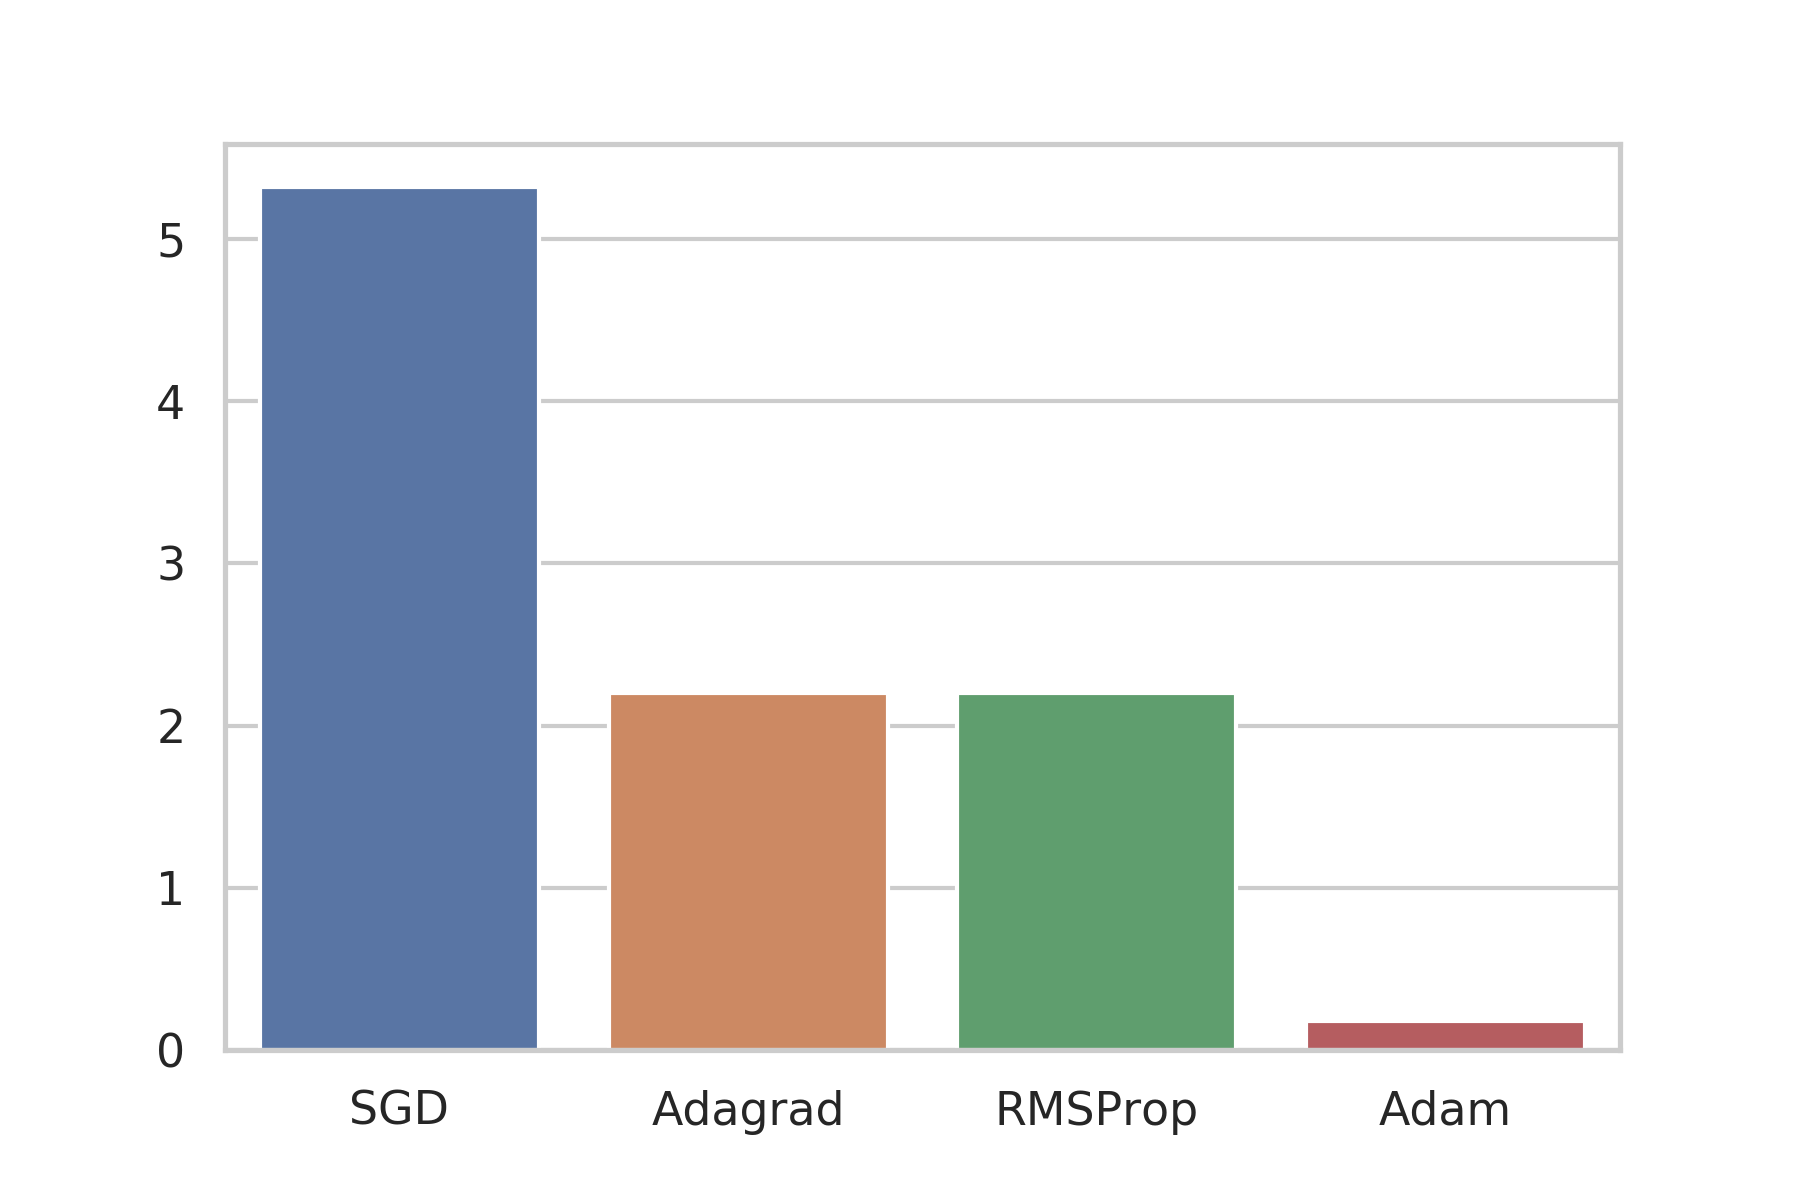
\includegraphics[width=.46\textwidth]{mainmatter/4-Results/images/Experiment_optimizer-MSE.png}
    } 
    \caption[Optimizer Chart: CI and MSE]{Bar Chart: Plot of concordance index (CI) and Mean Squared Error(MSE). Adam Optimizer~\ref{sub@fig:opt-ci} shows highest CI score and \ref{sub@fig:opt-mse} shows lowest MSE among all other optimizers. The worst is statistic gradient descent optimizer for protein-drug interaction prediction.}
    \label{fig:optimizer_plot}
\end{figure}

% Observing the table \ref{table:optimizer}, the calculations show that

\section{Analysis}
Table \ref{table:results} shows that the optimal filter window size under all settings can be chosen equal to 8 for both drugs and proteins. The highest C-Index Score of (87.30\%) was obtained under Setting 1 when both the drugs and proteins were present in the validation set and training set. This can also be better realized visually from Figure \ref{fig:ci_curve} and \ref{fig:ci_curve_2}.
 
\begin{figure}[tbp]\centering
    \subfloat[][Setting 1]{
        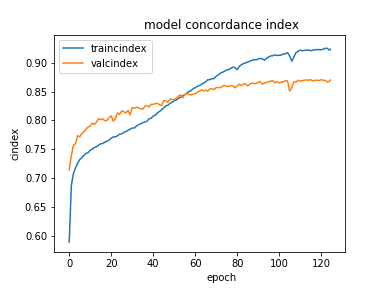
\includegraphics[width=.9\textwidth]{mainmatter/4-Results/images/S1_CI.png}
        \label{fig:s1_cindex}
    }
    \qquad
    \subfloat[][Setting 2]{
        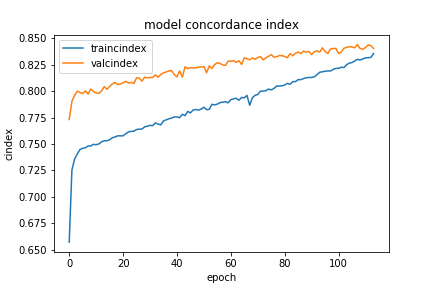
\includegraphics[width=.9\textwidth]{mainmatter/4-Results/images/S3_CI.png}
        \label{fig:s2_cindex}
    }
    \caption[Concordance Score during Training (a)]{Plot of Training-Validation C-Index Scores over various Settings: 
    \ref{sub@fig:s1_cindex} has highest score and \ref{sub@fig:s2_cindex} shows lowest score. Under S1 Setting, the epoch reaches the optimal value after 110 epochs after which the call back automatically stops training the model further. Under S2 Setting, the model validation loss does not improve after 35 epochs.
    }
    \label{fig:ci_curve}
\end{figure}

\begin{figure} \centering
    \qquad
    \subfloat[][Setting 3]{
        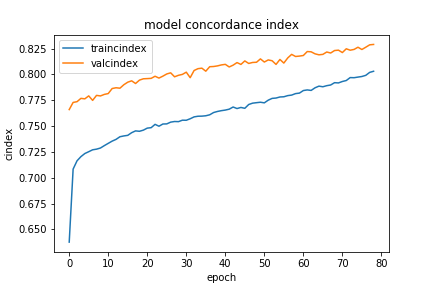
\includegraphics[width=.9\textwidth]{mainmatter/4-Results/images/S2_CI.png}
        \label{fig:s3_cindex}
    }
    \qquad
    \subfloat[][Setting 4]{
        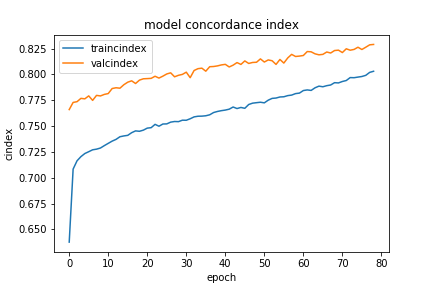
\includegraphics[width=.9\textwidth]{mainmatter/4-Results/images/S4_CI.png}
        \label{fig:s4_cindex}
    }
    \caption[Concordance Score during Training(b)]{ Plot of Training-Validation C-Index Scores over various Settings: \ref{sub@fig:s3_cindex} ranks 2\textsuperscript{nd} and \ref{sub@fig:s4_cindex} ranks the 3\textsuperscript{rd}. Setting S3 in Figure \ref{sub@fig:s3_cindex} was the most suitable training mode but it did not get good cindex score as to that of Setting S1 in Figure \ref{fig:s1_cindex}. Setting S4 in Figure \ref{sub@fig:s4_cindex} shows that the trainings being comparable to Setting S3. As expected both S3 and S4 missed one of their representative drug-protein pair during training.
    }
    \label{fig:ci_curve_2}
\end{figure}   

The comparison between the scores evaluated in same dataset has been compared and presented in table \ref{table:results_comparison} \citep{ozturk2018deepdta}. The benchmark dataset is publicly available in Journal of Chemical Information and Modeling \citep{Tang2013}.

\begin{table} [H]
    \centering
    \caption[Results Comparison]{Comparison of performace in prediction scores of protein-drug interaction problem. The performance of other algorithms is retrieved from literature~\citep{ozturk2018deepdta}. The method from this research is represented by FeatDTI. It performs the best amongst all the predictors, with the closest predictor being the DeepDTA.}
    \label{table:results_comparison}
    \begin{tabular}{|l|c|c|r|r|}
        \hline
        
        Methods & Proteins & Compounds & CI-Score & MSE \\ \hline
        KronRLS & Smith-Waterman & Pubchem Sim & 0.782 & 0.411 \\ \hline
        SimBoost & Smith-Waterman & Pubchem Simboost & 0.836 & 0.222 \\ \hline
        DeepDTA & CNN & CNN & 0.863 & 0.194 \\ \hline
        FeatDTI & CNN & CNN & \textbf{0.8730} & \textbf{0.177} \\ \hline
        
        \end{tabular}
\end{table}

\begin{figure}[H]
    \centering
    \subfloat[Actual Scores]{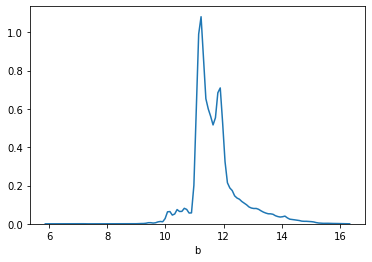
\includegraphics[width=.46\textwidth]{mainmatter/4-Results/images/train_y.png}
    \label{fig:train_actual}}
    \subfloat[Predicted Scores]{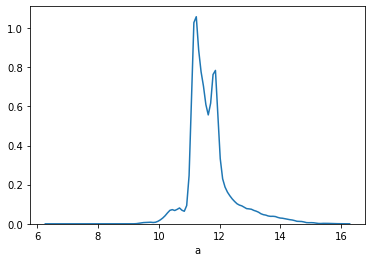
\includegraphics[width=.46\textwidth]{mainmatter/4-Results/images/pred_train_y.png}
    \label{fig:train_predict}
    } \qquad

    \subfloat[Difference of Actual and Predicted Scores]{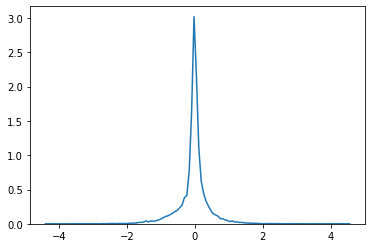
\includegraphics[width=.5\textwidth]{mainmatter/4-Results/images/train_diff.png}
    \label{fig:train_diff}}
    \caption[Training Results based on KIBA Score Prediction]{Kernel Density Estimation(KDE) plot of Training Results based on KIBA Score Prediction: The model evaluated the data set with actual KIBA scores~\ref{sub@fig:train_actual}. We obtain the predicted KDE of KIBA scores in~\ref{sub@fig:train_predict}. The differences in KIBA scores prediction and actual scores corresponding to same drug-protein pair is plotted in Figure~\ref{sub@fig:train_diff}.}
    \label{fig:pred_train}
\end{figure}

\begin{figure}
    \centering
    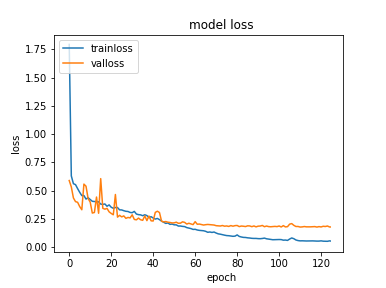
\includegraphics[width=1\textwidth]{mainmatter/4-Results/images/S1_loss.png}
    \caption[Training Loss Plot]{
        Training and Validation Loss Plot: Plot of Loss function of predicted values with training and validation set. The spikes were an unavoidable consequence of Mini-Batch Gradient Descent in Adam (batch size = 256). Some mini-batches have lossy data for optimization, inducing spikes during the initial phases of training. The loss plot was observed when trained with testing and validation drug-protein pair contained the drugs and proteins sequences used during the training phase. The filter size was 8 for both drugs and proteins. The loss function was stable with validation set and test data set around 115th epoch of training.
    }
    \label{fig:train_val_loss_plot}
\end{figure}

\iffalse

Similarly, the prediction scores and actual scores for validation sets  shown in Figure ~\ref{fig:val_train}


\begin{figure}[H]
    \subfloat[Testing Actual Scores]{
        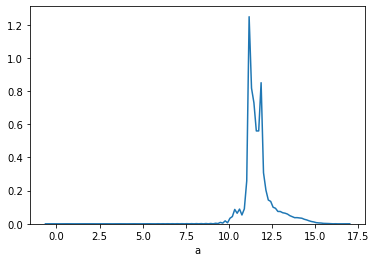
\includegraphics[width=.46\textwidth]{mainmatter/4-Results/images/val_y.png}
        \label{fig:actual_test}} \qquad
        \subfloat[Testing Predicted Scores]{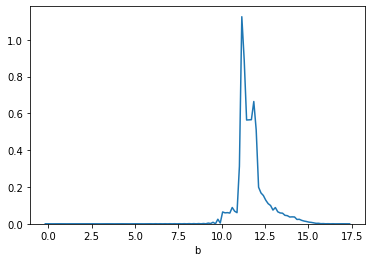
\includegraphics[width=.46\textwidth]{mainmatter/4-Results/images/pred_val_y.png}
    \label{fig:predict_test}
    } \qquad
    \subfloat[Testing Scores Difference]{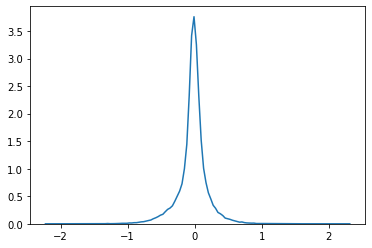
\includegraphics[width=.7\textwidth]{mainmatter/4-Results/images/val_difference.png}}
    \caption[Testing Results on KIBA score Prediction]{
        Kernel Density Estimation(KDE) plot of Testing (Validation) Results based on KIBA Score Prediction: The model evaluated the validation data set with actual KIBA scores~\ref{sub@fig:}. We obtain the predicted KDE of KIBA scores in~\ref{sub@fig:train_predict}. The differences in KIBA scores prediction and actual scores corresponding to same drug-protein pair is plotted in Figure~\ref{sub@fig:train_diff}.
    }
    \label{fig:val_train}
\end{figure}

\fi


\iffalse The similarity measures are evaluated using \citep{Cock2009}. \fi

\iffalse
The accuracy plots and cindex plots are shown in Figure ~\ref{fig:results}
\begin{figure}
    
\end{figure}

% Setting No. 4 Janahit
P1 = 0,  P2 = 0, P3 = 0, Fold = 2, CI-i = 0.804584, CI-ii = 0.803982, MSE = 0.412271
P1 = 0,  P2 = 0, P3 = 1, Fold = 2, CI-i = 0.807584, CI-ii = 0.805961, MSE = 1.510426
P1 = 0,  P2 = 1, P3 = 0, Fold = 2, CI-i = 0.816097, CI-ii = 0.815464, MSE = 1.614631
P1 = 0,  P2 = 1, P3 = 1, Fold = 2, CI-i = 0.787795, CI-ii = 0.787073, MSE = 0.485298
P1 = 0,  P2 = 0, P3 = 0, Fold = 1, CI-i = 0.829441, CI-ii = 0.829419, MSE = 0.529846
P1 = 0,  P2 = 0, P3 = 1, Fold = 1, CI-i = 0.805457, CI-ii = 0.805507, MSE = 0.810648
P1 = 0,  P2 = 1, P3 = 0, Fold = 1, CI-i = 0.816638, CI-ii = 0.817120, MSE = 0.922689
P1 = 0,  P2 = 1, P3 = 1, Fold = 1, CI-i = 0.829794, CI-ii = 0.829780, MSE = 0.271460
% Setting No. 2 alwaysgetwithanup
P1 = 0,  P2 = 0, P3 = 0, Fold = 0, CI-i = 0.788051, CI-ii = 0.789266, MSE = 0.678707
P1 = 0,  P2 = 0, P3 = 1, Fold = 0, CI-i = 0.802355, CI-ii = 0.802892, MSE = 0.360900
P1 = 0,  P2 = 1, P3 = 0, Fold = 0, CI-i = 0.803720, CI-ii = 0.806808, MSE = 0.792821
P1 = 0,  P2 = 1, P3 = 1, Fold = 0, CI-i = 0.803853, CI-ii = 0.805306, MSE = 0.672790
P1 = 0,  P2 = 0, P3 = 0, Fold = 1, CI-i = 0.823491, CI-ii = 0.821205, MSE = 0.526881
P1 = 0,  P2 = 0, P3 = 1, Fold = 1, CI-i = 0.815120, CI-ii = 0.815994, MSE = 0.302100
P1 = 0,  P2 = 1, P3 = 0, Fold = 1, CI-i = 0.842228, CI-ii = 0.840731, MSE = 0.226608
% Setting No. 3 MSCSKE
P1 = 0,  P2 = 0, P3 = 0, Fold = 2, CI-i = 0.815181, CI-ii = 0.815076, MSE = 1.562749
P1 = 0,  P2 = 0, P3 = 1, Fold = 2, CI-i = 0.805739, CI-ii = 0.806455, MSE = 1.541746
P1 = 0,  P2 = 1, P3 = 0, Fold = 2, CI-i = 0.813063, CI-ii = 0.813148, MSE = 1.259206
P1 = 0,  P2 = 1, P3 = 1, Fold = 2, CI-i = 0.824767, CI-ii = 0.825603, MSE = 1.396765
P1 = 0,  P2 = 0, P3 = 0, Fold = 1, CI-i = 0.811628, CI-ii = 0.810528, MSE = 0.679194
P1 = 0,  P2 = 0, P3 = 1, Fold = 1, CI-i = 0.811041, CI-ii = 0.811059, MSE = 2.034273

% Setting No. 1 MYSTIQUE
P1 = 0,  P2 = 0, P3 = 0, Fold = 1, CI-i = 0.813936, CI-ii = 0.811580, MSE = 0.893064
P1 = 0,  P2 = 0, P3 = 1, Fold = 1, CI-i = 0.810844, CI-ii = 0.809919, MSE = 1.285271
P1 = 0,  P2 = 1, P3 = 0, Fold = 1, CI-i = 0.873094, CI-ii = 0.873648, MSE = 0.177053
P1 = 0,  P2 = 1, P3 = 1, Fold = 1, CI-i = 0.807230, CI-ii = 0.806509, MSE = 1.056755
\fi